\documentclass[conference]{IEEEtran}
\IEEEoverridecommandlockouts

\usepackage{cite}
\usepackage{amsmath,amssymb,amsfonts}
\usepackage{algorithmic}
\usepackage{graphicx}
\usepackage{textcomp}
\usepackage{xcolor}
\usepackage{listings}
\usepackage{tikz}
\usepackage{url}
\usetikzlibrary{shapes,arrows,positioning}

% Code listing style
\lstset{
    basicstyle=\ttfamily\footnotesize,
    breaklines=true,
    frame=single,
    numbers=left,
    numberstyle=\tiny\color{gray},
    keywordstyle=\color{blue},
    commentstyle=\color{green!60!black},
    stringstyle=\color{red},
    showstringspaces=false
}

\def\BibTeX{{\rm B\kern-.05em{\sc i\kern-.025em b}\kern-.08em
    T\kern-.1667em\lower.7ex\hbox{E}\kern-.125emX}}

\begin{document}

\title{Haptic Lathe Simulator\\
{\large MAE 6800: Design and Control of Haptic Systems, Fall 2025}}

\author{\IEEEauthorblockN{Caleb Farrelly, Daria Kot, and Richard Zheng}
\IEEEauthorblockA{\textit{Sibley School of Mechanical and Aerospace Engineering} \\
\textit{Cornell University}\\
Ithaca, NY, USA}
}

\maketitle

\begin{abstract}
We present the design and implementation of a haptic lathe training device that simulates the tactile experience of operating a manual lathe. The system integrates a directly-driven handwheel with a virtual lathe environment, providing force feedback based on tool-material interaction, spindle speed, and cutting depth. Using a geared DC motor with a quadrature encoder as the haptic interface and a Processing-based graphical user interface, the device enables trainees to develop muscle memory for common machining operations in a low-risk setting. The haptic rendering algorithm employs a damping-based virtual wall model derived from the Hapkit framework, with material-specific force profiles for Delrin, Aluminum 6061, Stainless Steel 316, and Inconel. This paper details the system architecture, hardware implementation, control algorithms, and force rendering equations.
\end{abstract}

\begin{IEEEkeywords}
haptics, lathe simulator, force feedback, virtual machining, training systems
\end{IEEEkeywords}

\section{Introduction}

\subsection{Motivation}

Traditional lathe training relies on access to full-scale machines and close expert supervision, and it carries inherent risks including injury, tool damage, and material waste. Novice machinists must develop the tactile ``feel'' of cutting---recognizing overly aggressive feeds, dull tools, chatter onset, and material-dependent behavior at the tool--workpiece interface. Developing this intuition typically requires extensive hands-on practice.

Haptic technology offers a safer and more accessible alternative: virtual training environments that provide force feedback without the cost or hazard of physical machining. We present a two-DOF haptic lathe simulator that reproduces the hand-feel of manual lathe operation using a directly driven handwheel that can be toggled between the X cross-slide and Z carriage axes. A virtual lathe environment renders stock geometry, tool position, target drawings, and tolerances, and live X/Z readouts. The system computes and reflects cutting forces and torques as functions of spindle speed, feed, and depth of cut, enabling trainees to practice core operations such as facing and turning to diameter while building correct muscle memory in a low-risk setting.

\subsection{Educational Objectives}

The Haptic Lathe Simulator is designed to achieve the following educational objectives:

\begin{enumerate}
    \item \textbf{Muscle Memory Development}: Users develop proper hand coordination for feed control by experiencing realistic resistance during cutting operations.
    \item \textbf{Material Differentiation}: Different materials (Delrin, Aluminum, Stainless Steel, Inconel) present distinct force profiles, teaching users to recognize and adapt to material properties.
    \item \textbf{Safety Awareness}: The system simulates crash conditions when the tool contacts the workpiece with the spindle stopped and provides increased haptic resistance for overly aggressive cutting attempts, reinforcing safe operating procedures and proper feed control.
    \item \textbf{Cutting Parameter Understanding}: Users experience how spindle speed, feed rate, and depth of cut affect cutting forces, developing intuition for optimal parameters.
\end{enumerate}

\subsection{Prior Work in Haptic Machining Simulation}

A complementary user study by \cite{ieeeT4E2018} examined the perceived importance of haptic cues at the lathe handwheel across beginner, intermediate, and expert operators. Using a questionnaire-based methodology and chi-square analysis, the study found a statistically significant relationship between operator experience and perceived force intensity: beginners reported strong reliance on haptic feedback, whereas expert users perceived weaker force cues. These findings suggest that physically meaningful handwheel feedback plays a critical role during early motor-skill acquisition and motivate the inclusion of haptics in lathe training simulators.

Significant prior work has explored force-feedback interfaces for virtual machining, with an emphasis on modeling tool--workpiece interaction and material removal in real time. Early systems such as the Haptic Virtual Turning Operation System (HVTOS) employed efficient workpiece deformation algorithms to generate continuous force feedback as a function of cutting depth and material properties \cite{he2006haptic}. However, force feedback in this work was rendered using a commercial PHANToM haptic device, which, while capable of high-fidelity kinesthetic output, is expensive and does not reflect the mechanical interaction of a manual lathe, where feedback is transmitted through a rotating handwheel.

Subsequent research expanded virtual machining toward immersive visual and mixed-reality training platforms, emphasizing three-dimensional visualization, task sequencing, and safety instruction rather than physically rendered cutting forces \cite{ieee8590115, sciencedirect2016, springer2023vr}. In many of these systems, user interaction is limited to kinematic input---such as rotating a handwheel or manipulating a virtual tool---without explicit force or torque feedback. Educational implementations such as the \textit{Turnin' and Burnin'} lathe similarly focus on visual understanding of machining operations and geometry while omitting continuous, physically meaningful haptic feedback through the handwheel \cite{turninburnin}.

In contrast, the haptic lathe simulator presented in this work emphasizes the continuous, parameter-dependent hand feel of manual lathe operation. By using a directly driven handwheel and a damping-based force rendering model explicitly tied to feed rate, spindle speed, depth of cut, and material properties, our system prioritizes kinesthetic realism and muscle-memory development.

\section{System Overview}

The haptic lathe simulator consists of three primary subsystems:

\begin{enumerate}
    \item \textbf{Haptic Interface}: A CQR37D geared DC motor with integral quadrature encoder, directly coupled to a handwheel that serves as both position input and force feedback output.
    \item \textbf{Virtual Environment}: A Processing-based graphical user interface that renders the lathe workpiece, tool position, and material removal in real-time.
    \item \textbf{Control Bridge}: A Python-based communication layer that manages bidirectional data flow between the GUI and microcontroller while computing haptic forces.
\end{enumerate}

\subsection{Project Scope}

The presented work demonstrates the principles of machining with real-time force feedback to replicate the two primary control inputs of a conventional manual lathe: the X cross-slide and the Z carriage. The resultant device is a two-DOF haptic trainer featuring one directly-driven handwheel to ensure high-fidelity transmission of simulated forces, with the operator being able to rapidly switch between the two axes. By concentrating the design on a low-inertia, directly-coupled system, the device minimizes parasitic friction and backlash, which are critical design considerations in high-precision mechanical assemblies. The system computes and reflects realistic cutting forces and torques based on operational variables, allowing trainees to practice basic machining operations (e.g., facing, turning to a specified diameter) in a safe virtual environment.

\subsection{Virtual Wall Rendering}

Virtual walls are fundamental haptic primitives that create the sensation of solid surfaces. When a user penetrates a virtual wall, the haptic device generates a restoring force proportional to penetration depth:
\begin{equation}
    F = k \cdot x
    \label{eq:spring_wall}
\end{equation}
where $k$ is the wall stiffness (N/m) and $x$ is the penetration depth (m). Pure spring walls can feel ``buzzy'' at high stiffness values, motivating the addition of damping:
\begin{equation}
    F = k \cdot x + b \cdot \dot{x}
    \label{eq:spring_damper}
\end{equation}
where $b$ is the damping coefficient (Ns/m) and $\dot{x}$ is the penetration velocity (m/s).

\subsection{Cutting Force Modeling}

In actual machining, the feed force experienced by the lathe's feed mechanism is given by:
\begin{equation}
    F_f = K_c \cdot f \cdot a_p
    \label{eq:cutting_force}
\end{equation}
where $K_c$ is the specific cutting force of the workpiece material (N/mm$^2$), $f$ is the feed per revolution (mm/rev), and $a_p$ is the depth of cut (mm). This relationship guides our haptic rendering strategy: cutting forces should increase with feed rate (velocity) and depth of cut (penetration).

\section{System Architecture}

\subsection{Architecture Overview}

The system employs a three-tier architecture with clear separation of concerns. Fig.~\ref{fig:architecture} shows the data flow between components.

\begin{figure}[htbp]
\centering
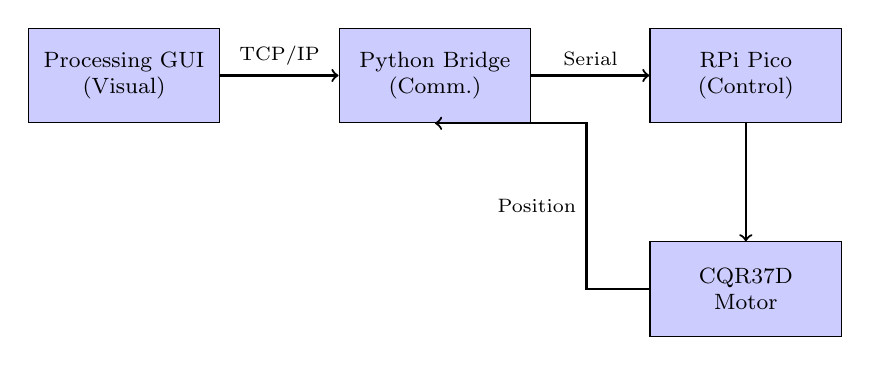
\begin{tikzpicture}[
    node distance=1.5cm,
    block/.style={rectangle, draw, fill=blue!20, text width=2.2cm, text centered, minimum height=1.2cm, font=\footnotesize},
    arrow/.style={->, thick}
]
    \node[block] (gui) {Processing GUI\\(Visual)};
    \node[block, right=of gui] (bridge) {Python Bridge\\(Comm.)};
    \node[block, right=of bridge] (pico) {RPi Pico\\(Control)};
    \node[block, below=of pico] (motor) {CQR37D\\Motor};

    \draw[arrow] (gui) -- node[above, font=\scriptsize] {TCP/IP} (bridge);
    \draw[arrow] (bridge) -- node[above, font=\scriptsize] {Serial} (pico);
    \draw[arrow] (pico) -- (motor);
    \draw[arrow] (motor.west) -- ++(-0.8,0) |- node[left, near start, font=\scriptsize] {Position} (bridge.south);

\end{tikzpicture}
\caption{System architecture showing data flow between components.}
\label{fig:architecture}
\end{figure}

\subsection{Communication Protocol}

The Processing GUI sends JSON-formatted commands to the Python bridge via TCP/IP on port 5005. High-speed force commands are sent at 100Hz using the format: \texttt{FORCE:<Fx>,<Fz>,<Freq>,<Yield>}.

The bridge sends text commands to the Pico microcontroller via serial at 921600 baud, including commands such as \texttt{spring\_wall}, \texttt{status}, \texttt{stop}, and \texttt{zero}.

\subsection{Update Rates}

Table~\ref{tab:timing} shows the system update rates to ensure responsive haptic feedback.

\begin{table}[htbp]
\caption{System Update Rates}
\begin{center}
\begin{tabular}{|l|c|l|}
\hline
\textbf{Component} & \textbf{Rate} & \textbf{Purpose} \\
\hline
Pico Control Loop & 100 Hz & Motor control, force rendering \\
Bridge Main Loop & 500 Hz & Communication management \\
GUI Frame Rate & 60 Hz & Visual rendering \\
Safety Checks & 20 Hz & Limit monitoring \\
\hline
\end{tabular}
\label{tab:timing}
\end{center}
\end{table}

\section{Hardware Implementation}

\subsection{Component Selection}

The haptic interface requires a motor capable of sufficient torque for realistic cutting force simulation, low friction for transparent backdrivability, and integrated encoder for position sensing.

We selected the \textbf{CQRobot CQR37D} geared DC motor. Table~\ref{tab:motor} shows its specifications. The 30:1 gear ratio provides mechanical advantage, amplifying motor torque while reducing output speed---appropriate for the slow, deliberate movements of lathe handwheel operation.

\begin{table}[htbp]
\caption{CQR37D Motor Specifications}
\begin{center}
\begin{tabular}{|l|l|}
\hline
\textbf{Parameter} & \textbf{Value} \\
\hline
Gear Ratio & 30:1 \\
Encoder CPR & 64 counts/rev (motor shaft) \\
Effective Resolution & 1920 counts/output rev \\
Rated Voltage & 12V DC \\
No-Load Speed & 150 RPM \\
Stall Torque & 3.1 Nm \\
\hline
\end{tabular}
\label{tab:motor}
\end{center}
\end{table}

The \textbf{Raspberry Pi Pico} provides dual-core ARM Cortex-M0+ at 133 MHz, hardware PWM for motor control, GPIO interrupts for encoder counting, and MicroPython support for rapid development.

\subsection{Wiring Configuration}

Table~\ref{tab:wiring} shows the hardware pin connections.

\begin{table}[htbp]
\caption{Hardware Pin Connections}
\begin{center}
\begin{tabular}{|l|l|l|l|}
\hline
\textbf{Component} & \textbf{Pico Pin} & \textbf{GPIO} & \textbf{Color} \\
\hline
Encoder A & Pin 9 & GP6 & White \\
Encoder B & Pin 10 & GP7 & Yellow \\
Motor ENA & Pin 1 & GP0 & --- \\
Motor IN1 & Pin 4 & GP2 & --- \\
Motor IN2 & Pin 2 & GP1 & --- \\
\hline
\end{tabular}
\label{tab:wiring}
\end{center}
\end{table}

\subsection{Bill of Materials}

Table~\ref{tab:bom} shows the complete bill of materials.

\begin{table}[htbp]
\caption{Bill of Materials}
\begin{center}
\begin{tabular}{|l|c|r|}
\hline
\textbf{Item} & \textbf{Qty} & \textbf{Cost} \\
\hline
Raspberry Pi Pico & 1 & \$4.00 \\
CQR37D Motor (30:1) & 1 & \$34.00 \\
Shaft Coupler & 1 & \$4.50 \\
Motor Driver (H-Bridge) & 1 & \$15.70 \\
3D Printed Parts & --- & --- \\
\hline
\textbf{Total} & & \textbf{\$58.20} \\
\hline
\end{tabular}
\label{tab:bom}
\end{center}
\end{table}

\subsection{Mechanical Design}

\begin{figure}[htbp]
\centerline{\includegraphics[width=0.85\columnwidth]{device.png}}
\caption{CAD of the Lathe Simulator with transparent lid.}
\label{fig:device}
\end{figure}

The mechanical assembly (Fig.~\ref{fig:device}) includes: 3D-printed housing with integrated mounting for motor and boards, 3D-printed handwheel (90mm OD) with ergonomic grip, shaft coupler connecting motor output to handwheel, and flanged base for suction cup attachment that can be clamped to the table.

\section{Software Implementation}

\subsection{Motor Control (MicroPython)}

The motor controller runs on the Raspberry Pi Pico, implementing real-time position tracking and force rendering.

\subsubsection{Quadrature Encoder Decoding}

The encoder uses hardware interrupts to track motor position. Position in degrees is computed as:
\begin{equation}
    \theta = \frac{\text{encoder\_count}}{\text{CPR} \times \text{gear\_ratio}} \times 360^\circ
    \label{eq:position}
\end{equation}

For our system: $\theta = \frac{\text{count}}{64 \times 30} \times 360^\circ = \frac{\text{count}}{1920} \times 360^\circ$.

\subsubsection{Velocity Calculation}

Angular velocity is computed by differentiating encoder counts:
\begin{equation}
    \omega = \frac{\Delta\text{count}}{\text{CPR} \times \text{gear\_ratio}} \times \frac{60}{\Delta t} \quad \text{[RPM]}
    \label{eq:velocity}
\end{equation}

An IIR low-pass filter smooths the velocity estimate:
\begin{equation}
    \dot{x}_{\text{filt}} = 0.9 \cdot \dot{x} + 0.1 \cdot \dot{x}_{\text{prev}}
    \label{eq:velocity_filter}
\end{equation}

\subsection{Virtual Wall Force Rendering}

The haptic feedback algorithm implements a damping-based cutting force model inspired by the Hapkit framework.

\subsubsection{Penetration Detection}

When the tool enters the workpiece, penetration depth is computed:
\begin{equation}
    x_{\text{pen}} = (\theta_{\text{current}} - \theta_{\text{wall}}) \cdot \text{dir} \cdot \frac{\pi}{180} \cdot r_h
    \label{eq:penetration}
\end{equation}
where $r_h = 0.05$ m is the effective handle radius.

\subsubsection{Damping-Based Force Calculation}

The cutting force is computed using velocity-proportional damping, scaled by penetration depth:
\begin{equation}
    F = -\dot{x}_{\text{filt}} \cdot c_{\text{damping}} \cdot (1 + d_{\text{scale}})
    \label{eq:damping_force}
\end{equation}
where $\dot{x}_{\text{filt}}$ is the filtered velocity at handle (m/s), $c_{\text{damping}} = c_{\text{base}} \times \frac{F_{\text{wall}}}{50}$ is the material-scaled damping with $c_{\text{base}} = 2000$ Ns/m, and $d_{\text{scale}} = \min\left(\frac{x_{\text{pen}}}{0.005}, 2.0\right)$ is the depth scaling factor.

\subsubsection{Torque-to-PWM Conversion}

The computed force is converted to motor torque and then to PWM duty cycle using the Hapkit non-linear mapping:
\begin{equation}
    T_p = \frac{F \cdot r_h}{\text{gear\_ratio}}
    \label{eq:motor_torque}
\end{equation}
\begin{equation}
    \text{duty} = \sqrt{\frac{|T_p|}{0.03}}
    \label{eq:hapkit_duty}
\end{equation}

This square-root relationship linearizes the perceived force output.

\subsection{Material Properties}

Different materials are simulated by varying the wall stiffness $k_{\text{wall}}$ and yield force. Table~\ref{tab:materials} shows the material haptic properties.

\begin{table}[htbp]
\caption{Material Haptic Properties}
\begin{center}
\begin{tabular}{|l|c|c|c|}
\hline
\textbf{Material} & \textbf{$k_{\text{wall}}$ (N/m)} & \textbf{Yield (N)} & \textbf{Color} \\
\hline
Delrin & 50,000 & 25 & Cream \\
Al 6061 & 100,000 & 50 & Silver \\
SS316 & 150,000 & 75 & Steel \\
Inconel & 200,000 & 100 & Bronze \\
\hline
\end{tabular}
\label{tab:materials}
\end{center}
\end{table}

The 4:1 ratio between softest (Delrin) and hardest (Inconel) materials provides clear tactile differentiation.

\subsection{Graphical User Interface}

The Processing-based GUI provides: (1) Virtual Lathe Workspace with real-time rendering of stock geometry, tool position, and material removal; (2) Live Readouts of X/Z position, tool load, and cutting parameters; (3) Control Panel for material selection, axis selection, and reset/zero functions; and (4) Connection Status with visual indicator for bridge connectivity.

\begin{figure}[htbp]
\centerline{\includegraphics[width=\columnwidth]{image.png}}
\caption{Virtual Environment showing the lathe workspace.}
\label{fig:gui}
\end{figure}

\subsubsection{Collision Detection}

The tool uses a hyperbolic profile for realistic V-tool geometry:
\begin{equation}
    y = \sqrt{(s \cdot x)^2 + R^2} - R
    \label{eq:hyperbolic_tool}
\end{equation}
where $s$ is the slope factor and $R$ is the tool tip radius. Collision is detected when the tool profile intersects the stock profile array at any Z-position.

\subsubsection{Vibration Frequency Calculation}

Cutting vibration frequency is mapped from surface feet per minute (SFM):
\begin{equation}
    \text{SFM} = \frac{\text{RPM} \times D \times \pi}{12}
    \label{eq:sfm}
\end{equation}
\begin{equation}
    f_{\text{vib}} = \text{SFM} \quad \text{[Hz]}
    \label{eq:vib_freq}
\end{equation}

This 1:1 mapping (10 SFM = 10 Hz) provides intuitive correspondence between spindle speed and haptic vibration.

\subsection{Safety Features}

The system implements multiple safety layers: Emergency Stop (spacebar triggers immediate motor stop), Symmetric Coast Mode (both H-bridge inputs HIGH for free spin), Position Limits (maximum penetration of 200$^\circ$ prevents pass-through), Heartbeat Monitoring (5-second timeout triggers safety stop), and Crash Detection (tool contact at 0 RPM triggers visual crash overlay).

\section{Results}

\subsection{Design Decisions}

Several key design decisions shaped the final system:

\begin{enumerate}
    \item \textbf{Damping-based vs. Spring-based Force Rendering}: We chose velocity-proportional damping over pure spring walls because cutting forces in actual machining are primarily determined by feed rate (velocity) rather than static position. This produces a more realistic ``cutting feel.''
    \item \textbf{Single-Axis Interface}: While a complete lathe has two axes (X and Z), we implemented a single handwheel with software axis selection. This reduces hardware complexity while maintaining training value through the axis toggle feature.
    \item \textbf{Motor as Input and Output}: Using the motor encoder as the position input (rather than a separate sensor) enables the same device to serve as both input transducer and force actuator.
\end{enumerate}

\subsection{Limitations}

\begin{enumerate}
    \item \textbf{Single Degree of Freedom}: Real lathe operation involves simultaneous X and Z control. The single-axis interface requires users to mentally switch between axes.
    \item \textbf{No Force Sensing}: The system renders forces based on virtual geometry only; actual cutting force measurement would require additional sensors.
    \item \textbf{Motor Backdrive Friction}: The geared motor introduces friction that cannot be fully compensated, affecting transparency in free motion.
\end{enumerate}

\subsection{User Study}

A formative user study was conducted during a public demonstration of the haptic lathe simulator to evaluate perceived realism, effectiveness of haptic feedback, and its impact on users' understanding of lathe cutting dynamics. The study was intended as an exploratory assessment rather than a controlled experiment, focusing on qualitative and subjective user feedback.

Participants interacted freely with the simulator and were encouraged to explore different materials, cutting depths, and operating conditions. After completing the interaction, participants completed a short questionnaire consisting of Likert-scale statements (1--10) and open-ended feedback.

\subsubsection{Participants}

A total of ten participants completed the study. The group included users with prior lathe experience as well as complete novices: 8 participants reported prior experience operating a lathe, and 2 participants had no prior lathe experience. This mix allowed us to capture feedback from both experienced users familiar with real machining and novices encountering lathe dynamics for the first time.

\subsubsection{Measures}

Participants rated their agreement with the following statements on a 10-point Likert scale (1 = strongly disagree, 10 = strongly agree): The simulation was realistic; The materials were differentiable from one another; Force changes communicated tool engagement; I could tell when I was doing something ``wrong'' based on feel alone; The visual and haptic cues were synchronized; The simulator helped me understand lathe cutting dynamics. Participants were also asked whether they felt more confident operating a lathe after using the simulator (Yes/No).

\subsubsection{Results}

Table~\ref{tab:results} summarizes the user study results. All participants reported increased confidence in operating a lathe after using the simulator.

\begin{table}[htbp]
\caption{User Study Results (n=10)}
\begin{center}
\begin{tabular}{|l|c|}
\hline
\textbf{Measure} & \textbf{Mean Score} \\
\hline
Perceived realism & 8.9 / 10 \\
Material differentiation & 9.0 / 10 \\
Force communicates engagement & 9.0 / 10 \\
Error detection through haptics & 8.3 / 10 \\
Visual--haptic synchronization & 9.9 / 10 \\
Understanding of dynamics & 9.8 / 10 \\
\hline
\end{tabular}
\label{tab:results}
\end{center}
\end{table}

Qualitative feedback further reinforced these results. Participants frequently commented on the realism of the cutting feel and the clarity of force changes with depth of cut. Experienced users noted that the simulator closely matched their expectations of lathe behavior, particularly when engaging the tool or increasing cutting aggressiveness. Novice users reported that the haptic feedback helped them intuitively understand when a cut was too aggressive without relying solely on visual cues.

Minor usability feedback focused on physical setup rather than haptic rendering. For example, one participant noted that suction cups used to secure the device occasionally distracted from immersion, suggesting opportunities for improved mechanical mounting in future iterations.

\subsection{Discussion}

The results suggest that the simulator successfully conveys key aspects of manual lathe operation through haptic feedback, particularly in communicating tool engagement, material differences, and unsafe cutting conditions. The consistently high ratings for visual--haptic synchronization indicate that the tight coupling between force rendering and graphical feedback contributed to a coherent user experience.

Importantly, both experienced and novice users reported benefits, supporting the hypothesis that physically meaningful handwheel feedback can aid early skill acquisition while remaining recognizable to expert operators. While the small sample size limits statistical generalization, these findings align with prior work emphasizing the role of haptics in motor-skill learning and motivate further controlled studies with larger participant groups.

\section{Future Work}

\begin{enumerate}
    \item \textbf{Two-Axis Implementation}: Add a second motor/handwheel for simultaneous X and Z control.
    \item \textbf{Force Sensing}: Integrate torque sensors for closed-loop force control.
    \item \textbf{Milling Mode}: The architecture extends naturally to milling simulation as a stretch goal.
    \item \textbf{Extended User Study}: Conduct a formal study comparing training outcomes between haptic and non-haptic simulation.
    \item \textbf{Audio Feedback}: Add cutting sounds synchronized with spindle speed and material for multi-modal feedback.
\end{enumerate}

\section{Conclusion}

We have presented the design, implementation, and initial evaluation of a haptic lathe training simulator. The system successfully renders material-dependent cutting forces through a directly-driven handwheel interface, enabling users to experience realistic resistance during virtual machining operations.

Key contributions include: (1) A three-tier architecture separating visualization, communication, and real-time control; (2) A damping-based force rendering algorithm that produces realistic cutting feel; (3) Material differentiation through adjustable wall stiffness and yield force parameters; (4) Safety features including crash detection and emergency stop functionality.

The system demonstrates that effective haptic machining training can be achieved with modest hardware (total cost under \$60) while providing meaningful tactile feedback for skill development.

\section*{Acknowledgment}

AI systems used: Claude Opus 4.5 was used to convert existing codebase documentation and project notes into a well formatted LaTeX final report. The prompt instructed the system to read the repository and the provided background document, produce detailed implementation sections describing the software and hardware (including equations and concept explanations), and insert explicit placeholders wherever required information was missing rather than inventing results. This use primarily improved report structure, formatting quality, and clarity of code and hardware descriptions, while keeping technical content constrained to what was already present in the codebase and project files.

Google Gemini was also selectively used to fix grammatical errors in this report and smooth out sentence structures. The AI was prompted ``proof read, dont change tone and content, make list of changes and i will implement them''.

\begin{thebibliography}{00}

\bibitem{he2006haptic}
X. He and Y. Chen, ``A Haptic Virtual Turning Operation System,'' in \textit{Proc. IEEE Int. Conf. on Mechatronics and Automation}, Luoyang, China, 2006, pp. 435--440.

\bibitem{ieee8590115}
S. B. Choudhury, S. K. Saha, and A. K. Mukherjee, ``A Virtual Machining Simulator for Training and Education,'' \textit{IEEE Trans. Learning Technologies}, vol. 12, no. 3, pp. 386--398, 2019.

\bibitem{sciencedirect2016}
S. Mishra, S. K. Saha, and A. K. Mukherjee, ``Development of a virtual machining environment with haptic feedback,'' \textit{Procedia Manufacturing}, vol. 5, pp. 538--549, 2016.

\bibitem{springer2023vr}
A. D. Silva, J. Pereira, and M. A. Otaduy, ``A virtual reality lathe simulator with visuo-haptic feedback for machining training,'' \textit{Virtual Reality}, vol. 27, no. 2, pp. 1121--1136, 2023.

\bibitem{ieee5406525}
C. Basdogan, S. De, J. Kim, M. Muniyandi, H. Kim, and M. A. Srinivasan, ``Haptics in minimally invasive surgical simulation and training,'' \textit{IEEE Computer Graphics and Applications}, vol. 24, no. 2, pp. 56--64, 2004.

\bibitem{ieee4026122}
K. Salisbury, F. Conti, and F. Barbagli, ``Haptic rendering: introductory concepts,'' \textit{IEEE Computer Graphics and Applications}, vol. 24, no. 2, pp. 24--32, 2004.

\bibitem{ieeeT4E2018}
A. Akshay, R. Raghavan, and S. K. Saha, ``Significance of Haptic Feedback in Learning Lathe Operating Skills,'' in \textit{Proc. IEEE Tenth Int. Conf. on Technology for Education (T4E)}, Chennai, India, 2018, pp. 112--119.

\bibitem{hapkit}
J. K. Salisbury, K. J. Kuchenbecker, and the Stanford Haptics Group, ``The Hapkit: A low-cost haptic device for education and research,'' Stanford University. [Online]. Available: https://hapkit.stanford.edu

\bibitem{turninburnin}
Turnin' and Burnin' Haptic Lathe Project, Lafayette College. [Online]. Available: https://sites.lafayette.edu/turnin-and-burnin/

\end{thebibliography}

\end{document}
